\documentclass[12pt]{article}

\input{C:/Users/ilden/Documents/School/TeX памятка/header.tex}

\begin{document}
	\tableofcontents
	\setcounter{tocdepth}{3}
	\newpage
	\section{Биология.}
	\begin{xltabular}{\textwidth}{|p{3cm}|X|p{3cm}|}
		\hline
		Направление & ОХ & Ученный \\
		\hline
		Классическое. & Изучает многообразие живой природы. Наблюдает и анализирует все в живой природе. & Гиппократ, Аристотель, Теофраст. \\
		\hline
		Эволюционное. & Изучает эволюцию живых организмов. Объяснение органического разнообразия природы. & Дарвин, Шлейден, Опарин, Ламарк. \\
		\hline
		Физико-химическое. & Изучение с использованием новых физико-химических методов и знаний. & Мечников, Пастер, Кох, Гарвей. \\
		\hline
	\end{xltabular}
	\begin{xltabular}{\textwidth}{|p{3.8cm}|X|p{3cm}|}
		\hline
		Метод & ОХ & Ученый \\
		\hline
		Описание. & Наблюдение и фиксирование фактического материала. Самый древний. Основной метод примерно до $18$ века. & Гиппократ, Аристотель, Теофраст. \\
		\hline
		Сравнение. & Сходства и различия организмов. Данные для систематизации. & Аристотель, Ламарк, Бэр. \\
		\hline
		Исторический. & Осмысление факторов по предыдущем результатам. & Дарвин, Ламарк. \\
		\hline
		Экспериментальный. & Изучение при помощи опытов. Дополнительные вспомогательные инструменты. & Гарвей, Мендель, Матье Бал, Кох. \\
		\hline
	\end{xltabular}
	\subsection{Свойства живого.}
	\begin{itemize}
		\item Обмен веществ (дыхание, пищеварение).
		\item Раздражимости (реакция на окружающую среду).
		\item Рост (количественное) и развитие (качественное).
		\item Размножение.
		\item Единство химического состава (основные~--- $C, O, H, N$).
		\item Структурная организация.
		\item Открытость.
		\item Наследственность и изменчивость.
		\item Саморегуляция.
	\end{itemize}
	\subsection{Уровни организации живой материи.}
	Молекулярный уровень~--- вирусы. Клеточный~--- бактерии. Организменный~--- одно- и многоклеточные. Популяционно-видовой. Экосистемный. Биосферный.
	\section{Клетка.}
	\begin{itemize}
		\item Наименьшая структурная единица.
		\item Наименьшая функциональная единица.
	\end{itemize}
	\subsection{Клеточная теория.}
	\begin{person}
		Роберт Гук. Первый микроскоп. Ввел понятие "клетка".
	\end{person}
	\begin{person}
		Антони ван Левенгук, XVI век. Первый микроскоп с увеличением в $300$ раз.
	\end{person}
	\begin{person}
		Шлейден и Шванн, XIX век. Положения клеточной теории. Ошибка в том, что не было объяснено откуда появляются клетки (считали, что появились из неклеточного вещества).
	\end{person}
	\begin{person}
		Мечников, конец XIX века. Фагоцитоз (процесс, когда клетки захватывают и переваривают твердые частицы).
	\end{person}
	\subsection{Молекулярный уровень.}
	Химические элементы:
	\begin{itemize}
		\item Макро; до $\dfrac{1}{100}$; основные~--- $C, O, H, N$.
		\item Микро; от $\dfrac{1}{1000}$ до $\dfrac{1}{1000000}$.
		\item Ульра-микро.
	\end{itemize}
	\subsection{Вещества клетки.}
	\begin{itemize}
		\item Органические (большая часть органики~--- белки).
		\item Неорганические (преобладают из-за воды).
	\end{itemize}
	\subsubsection{Вода.}
	\begin{xltabular}{\textwidth}{|p{3.5cm}|X|X|}
		\hline
		Свойство & ОХ & Пример \\
		\hline
		Растворитель. & Легко растворяет ионные соединения (соли, кислоты, основания); некоторые не ионные, но полярные соединения. Вещества, хорошо растворимые в воде~--- гидрофильные, плохо~--- гидрофобные. Благодаря полярности и водородных связях. & Кислород, углекислый газ. \\
		\hline
		Теплоемкость. & Способность поглощать тепловую энергию при минимальном повышении собственной температуры. & Защищает ткани от быстрого и сильного повышения температуры. Охлаждение с помощью выделения воды. \\
		\hline
		Теплопроводность. & Обеспечение равномерного распределения температуры. & Высокая удельная теплоемкость и высокая теплопроводность делают воду идеальной жидкостью для поддержания теплового равновесия клетки и организма. \\
		\hline
		Сжимаемость. & Практически не сжимается. Создает тургорное давление, определяя объем и упругость клеток и тканей. & Гидростатический скелет поддерживает форму у круглых червей, медуз и других. \\
		\hline
		Поверхностное натяжение. & Возникает благодаря образованию водородных связей между молекулами воды и молекулами других веществ. & Капилярный кровоток, восходящий и нисходящий токи растворов в растениях. \\
		\hline
	\end{xltabular}
	\section{Минеральные вещества.}
	\begin{xltabular}{\textwidth}{|X|X|X|}
		\hline
		Свойство & Химический элемент & ОХ \\
		\hline
		Кристаллические включения. & Слаборастворимые соли кальция и фосфора. & Образование опорных структур клетки, например вещества костных ткани у моллюсков. \\
		\hline
		Проводимость. & Катионы и Анионы минеральных веществ. & Разность потенциалов из-за различной концентрации. \\
		\hline
		Кислотность. & Ионы $H^+$. & Нейтральные, кислотные, основные. Определяют кислотную среду. \\
		\hline
		Буферные системы. & $HPO_4^{2-}$, $H_2PO_4^-$, $H_2CO_3$, $HCO_4^-$. & Поддерживает постоянство $pH$ в клетках. \\
		\hline
		Синтез. & Соединения азота, фосфора, кальция и другие неорганические вещества. & Синтез белков, аминокислот, нуклеиновых кислот. \\
		\hline
	\end{xltabular}
	\section{Органические вещества.}
	\subsection{Углеводы.}
	Углеводы ($C_n(H_2O)_m$):
	\begin{itemize}
		\item Моносахариды
		\item Олигосахариды
		\item Полисахариды
	\end{itemize}
	Сахариды так как большинство хорошо растворимы в воде; сладкие. \\
	С увеличением количества мономеров растворимость полисахаридов уменьшается и исчезает сладкий вкус. \\
	Углеводы являются первичным продуктом фотосинтеза. \\
	Углеводы есть во всех клетках.
	\begin{xltabular}{\textwidth}{|X|X|X|}
		\hline
		Группа & Пример & Особенность \\
		\hline
		Моносахариды. & Рибоза, глюкоза, фруктоза, дезоксирибоза, галактоза. & Имеют сладкий вкус, бесцветные, кристаллические, растворимые, во всех клетках, являются мономерами. \\
		\hline
		Олигосахариды. & Сахароза, мальтоза, лактоза & Образованы двумя или более моносахаридами. Также растворимы в воде и имеют сладковатый вкус. Связаны ковалентно друг с дургом. \\
		\hline
		Полисахариды. & Хитин, крахмал, гликоген, целлюлоза. & Полимеры. Состоят из неопределенного большого числа остатков молекул моносахаридов. \\
		\hline
	\end{xltabular}
	\begin{xltabular}{\textwidth}{|X|X|X|}
		\hline
		Функция & Пример углевода & Характеристика \\
		\hline
		Энергетическая. & Моносахариды (глюкоза). & При ферментативном расщеплении и окислении молекул углеводов выделяется энергия, которая обеспечивает жизнедеятельность организма. При полном расщеплении $1$г углеводов высвобождает $17.6$кДж энергии. \\
		\hline
		Запасающая. & Полисахариды (крахмал и гликоген). & При избытке они накапливаются в клетке в качетсве запасающих веществ и при необходимости используется организмом как источник энергии. \\
		\hline
		Структурная/строительная. & Целлюлоза, хитин. & Строительный материал. В среднем $20$--$40\%$ материала клеточных стенок составляет целлюлоза. \\
		\hline
		Защитная. & Камеди $\rightarrow$ производный моносахаридов. & Препятствуют проникновению в раны болезнетворных микроорганизмов. Твердые клеточные стенки одноклеточных и хитиновые покровы членистоногих. \\
		\hline
	\end{xltabular}
	\subsection{Липиды или жиры.}
	Молекул жира состоит из глицерина и трех остатков жирной кислоты. Иногда вместо остатка жирной кислоты могут быть белки, углеводы или остатки фосфорной кислоты. \\
	Более $600$ жиров. $180$~--- животных, $420$~--- растительных. \\
	Жиры бывают:
	\begin{itemize}
		\item Протоплазменный.
		\item Резервный.
	\end{itemize}
	\begin{xltabular}{\textwidth}{|X|X|X|}
		\hline
		Функция & Пример & Характеристика \\
		\hline
		Энергетическая & Триглицериды (жиры и масла) & Основная функция. При окислении 1 г жира выделяется около 38,9 кДж (9,3 ккал) энергии, что более чем в два раза превышает энергетическую ценность углеводов или белков. Жиры служат основным запасом энергии в организме. \\
		\hline
		Структурная (строительная) & Фосфолипиды, холестерин & Образование клеточных мембран. Фосфолипиды формируют липидный бислой всех клеточных мембран, обеспечивая их текучесть и избирательную проницаемость. Холестестрол стабилизирует мембрану, придавая ей жесткость. \\
		\hline
		Запасающая & Триглицериды (в жировой ткани) & Создание резервов энергии. Жиры запасаются в подкожной клетчатке, сальнике и вокруг внутренних органов. Жировые запасы также обеспечивают механическую защиту (амортизация) и термоизоляцию. \\
		\hline
		Регуляторная (гормональная) & Стероидные гормоны (половые гормоны, кортикостероиды), эйкозаноиды (простагландины) & Липиды выступают в роли гормонов и сигнальных молекул. Стероиды регулируют обмен веществ, репродуктивную функцию, стрессовые реакции. Эйкозаноиды регулируют воспаление, боль, температуру тела, артериальное давление. \\
		\hline
		Защитная и теплоизоляционная & Триглицериды (подкожный жир) & Защита от механических повреждений и потерь тепла. Жировая прослойка смягчает удары и защищает внутренние органы. Благодаря низкой теплопроводности жир помогает сохранять тепло организма (особенно важно у морских млекопитающих). \\
		\hline
		Источник метаболической воды & Триглицериды & При окислении жиров образуется вода. Из 100 г жира получается около 107 мл воды. Это особенно важно для животных пустыни (верблюды, тушканчики) и впадающих в спячку (сурки, медведи). \\
		\hline
		Каталитическая (ферментативная)	& Жирорастворимые витамины (A, D, E, K) & Витамины-липиды являются коферментами или предшественниками коферментов. Например, витамин А входит в состав зрительного пигмента родопсина; витамин К необходим для синтеза факторов свертывания крови. \\
		\hline
		Улучшение вкуса пищи и насыщения & Триглицериды & Жиры улучшают вкусовые качества пищи и продлевают чувство сытости, так как они медленно перевариваются и подавляют секрецию желудочного сока. \\
		\hline
	\end{xltabular}
	\subsection{Белки.}
	Белок~--- полимерная молекула. Его мономером является аминокислота ($20$ штук). Белки $=$ протеины $=$ полипептиды.
	\paragraph{Аминокислота.} Общая формула: $NH_2 - CH (R) - COOH$. По радикалу ($R$) определяем аминокислоту. $NH_2$~--- $N$-конец аминокислоты, $COOH$~--- $C$-конец аминокислоты. \\
	\subsubsection{Структура белка.}
	\begin{enumerate}
		\item Первичная структура белка в виде цепочки; индивидуальна для каждого белка. Очень большая, поэтому клетки не удобно.
		\item Вторичная структура белка в виде спирали. Удерживается водородными связями.
		\item Третичная (глобал). Спираль упаковывается в шарик. Образуется за счет связей внутри радикалов.
		\item Четвертичная. Несколько глобал, соединенных между собой. Характерна только для белков с очень важной функцией.
	\end{enumerate}
	\begin{definition}
		Денатурация~--- разрушение структуры белка. Ренатурация~--- восстановление структуры белка (возможна, если белок не утратил первичную структуру).
	\end{definition}
	\begin{xltabular}{\textwidth}{|X|X|X|}
		\hline
		Функция & Пример & Характеристика \\
		\hline
		Структурная (опорная) & Коллаген, кретин & Образуют волокна и сети, обеспечивающие прочность и эластичность тканей. Коллаген — основа соединительной ткани (сухожилия, хрящи), кератин — основной белок волос, ногтей, перьев. \\
		\hline
		Ферментативная (каталитическая) & Амилаза, пепсин, РНК-полимераза & Биологические катализаторы (ферменты), которые в тысячи раз ускоряют химические реакции в клетке. Амилаза расщепляет крахмал, пепсин — белки в желудке. \\
		\hline
		Транспортная & Гемоглобин, транспортные белки мембраны & Связывают и переносят различные вещества. Гемоглобин переносит кислород в крови. Белки-переносчики в мембранах транспортируют ионы и молекулы. \\
		\hline
		Защитная & Антитела (иммуноглобулины), фибриноген & Распознают и обезвреживают чужеродные объекты (вирусы, бактерии). Фибриноген участвует в свёртывании крови, предотвращая кровопотерю. \\
		\hline
		% Двигательная (сократительная) & Актин, миозин & Образуют сократимые структуры в мышечных волокнах, обеспечивая движение (мышцы, движение органелл внутри клетки). \\
		% \hline
		Регуляторная & Инсулин, гормон роста & Белки-гормоны регулируют обмен веществ и физиологические процессы. Инсулин, например, регулирует уровень глюкозы в крови. \\
		\hline
		% Рецепторная (сигнальная) & Белки-рецепторы (например, родопсин в сетчатке) & Расположены в мембранах клеток, принимают сигналы (свет, гормоны) из внешней среды и передают их внутрь клетки. \\
		% \hline
		% Запасающая (резервная) & Казеин (в молоке), яичный альбумин & Накопление питательных веществ для последующего использования организмом или зародышем. \\
		% \hline
		Энергетическая & Любой белок (в крайних случаях) & При недостатке углеводов и жиров белки могут расщепляться для получения энергии (при этом выделяется около $17,6$ $\frac{\text{кДж}}{\text{г}}$). \\
		\hline
	\end{xltabular}
	\subsection{Нуклеиновые кислоты.}
	Нуклеиновые кислоты~--- полимеры, их мономеры~--- нуклеотиды.
	\subsubsection{Основные нуклеиновые кислоты.}
	ДНК и РНК. Их состав: фосфатная группа, пентозный сахар и азотистое основание.
	\begin{xltabular}{\textwidth}{|X|X|X|}
		\hline
		Признак & ДНК & РНК \\
		\hline
		Название & Дезоксирибонуклеиновая кислота & Рибонуклеиновая кислота \\
		\hline
		Белок & Дезоксирибоза & Рибоза \\
		\hline
		Основание & Аденин ($2$ водородные связи), гуанин ($3$), цитозин ($3$), \textit{тимин} ($2$) & Аденин ($2$), гуанин ($3$), цитозин ($3$), \textit{урацил} ($2$) \\
		\hline
		Водородные связи & Постоянные & Временные \\
		\hline
		Внешний вид & Спираль. $5$'-конец (фосфатная группа) и $3$'-конец (пентозный сахар) & Также $3$'- и $5$'- концы \\
		\hline
		Местоположение & Ядро клетки, митохондрии, пластиды & Цитоплазма, рибосома, ядро, митохондрии, пластиды \\
		\hline
	\end{xltabular}	\begin{figure}[H]
		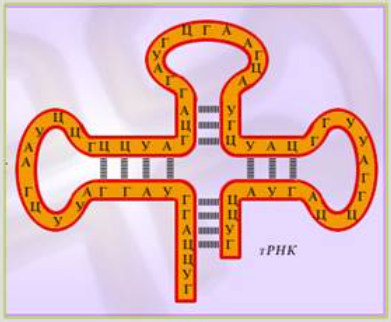
\includegraphics[height=0.25\textwidth]{extra-materials/тРНК}
		\caption{транспортная РНК}
	\end{figure}
	\begin{xltabular}{\textwidth}{|p{1.5cm}|p{1.5cm}|X|X|X|}
		\hline
		Название & Процент & Местоположение & ОХ & Функция \\
		\hline
		иРНК (мРНК) & $1-5\%$ & Ядро (в процессе синтеза), цитоплазма, рибосомы & Одноцепочечная молекула, образующаяся в процессе транскрипции на матрице ДНК. Имеет самую большую длину среди РНК. Нестабильна. & Перенос генетической информации от ДНК в ядре к рибосомам в цитоплазме, где служит матрицей для синтеза белка. \\
		\hline
		тРНК & $10-15\%$ & Цитоплазма, рибосомы & Небольшая молекула ($70-90$ нуклеотидов), имеющая сложную пространственную структуру ("клеверный лист"). Имеет участок для присоединения аминокислоты (акцепторный стебель) и антикодон. & Транспорт специфических аминокислот к растущей полипептидной цепи на рибосоме. Узнаёт свой кодон в иРНК благодаря антикодону. \\
		\hline
		рРНК & $80-85\%$ & Синтезируется в ядрышке, составляет основу рибосом & Самый распространённый тип РНК. Составляет вместе с белками субъединицы рибосом. Имеет сложную вторичную и третичную структуру. & Структурная (является каркасом рибосомы) и каталитическая (рибозимы): обеспечивает связывание рибосомы с иРНК, катализирует образование пептидных связей между аминокислотами. \\
		\hline
	\end{xltabular}
	\subsection{АТФ.}
	Аденозинтрифосфат.
	\subsubsection{Состав.}
	Аденин + рибоза + три остатка фосфорной кислоты (именно они определяют свойства АТФ; между ними макроэргическая связь). При отделении третьего и второго остатка фосфорной кислоты (разрушение макроэргической связи) выделяется до $40$ кДж энергии. При отделении первого остатка от углевода выделяется $14$ кДж.
	\subsubsection{Синтез АТФ.}
	Синтез проходит в митохондриях. Аденозинмонофосфат (АМФ) $\rightarrow$ аденозиндифосфат (АДФ) $\rightarrow$ аденозинтрифосфат (АТФ).
	\subsection{Витамины.}
	Открыты Луниным в $1880$ году. Термин "Витамины" введен в $1912$ году Функом. \\
	Суточная доля витаминов мала, они не заменяемые и не синтезируются.
	\subsubsection{Виды.}
	\begin{itemize}
		\item Водорастворимые. Основные: $C, B, PP, H$.
		\item Жирорастворимые. Основные: $A, D, E, K$.
	\end{itemize}
	\subsection{Сравнение АТФ, ДНК, РНК.}
	Сходства: общее строение, аналогичное местоположение.
	\section{Клеточный уровень.}
	Клетки есть у животных, растений, грибов, бактерий. \\
	Клетка~--- наименьшая структурная и функциональная единица. \\
	Науки~--- цитология, молекулярная биология, биохимия. \\
	\begin{xltabular}{\textwidth}{|X|X|X|}
		\hline
		Часть & ОХ & функция \\
		\hline
		Цитоплазма. & Основное вещество~--- гиалоплазма. Представляет собой густой бесцветный коллоидный раствор органических и неорганических веществ. Основа гиалоплазмы~--- вода ($70-90\%$ от массы), в ней много белков, обнаруживаются также липиды и различные неорганические соединения. Цитоплазма постоянно перемещается внутри клетки. & В ней протекают процессы обмена веществ в клетке, через нее происходит взаимодействие ядра и органоидов. \\
		\hline 
		Клеточная мембрана. & Толщина $8-12$ нМ. Универсальная биологическая мембрана, окружающая клетку. Имеет жидкомозаичную структуру: двойной слой липидов, в который погружены белки. Углеводы образуют гликокаликс~--- наружный слой. Обладает избирательной проницаемостью. & \begin{enumerate}
			\item Барьерная: Отделяет содержимое клетки от внешней среды, защищает от повреждений.
			\item Транспортная: Обеспечивает избирательный перенос веществ в клетку и из нее (диффузия, осмос, активный транспорт, эндо- и экзоцитоз).
			\item Рецепторная: Белки-рецепторы принимают сигналы из внешней среды (например, гормоны), обеспечивая коммуникацию с другими клетками.
			\item Структурная (опорная): Придает клетке форму, служит местом прикрепления цитоскелета.
		\end{enumerate} \\
		\hline
		Генетический аппарат. & Центр управления клетки; локализовано более $90\%$ ДНК. Обычно имеет шаровидную форму. Отделен от цитоплазмы оболочкой, состоящей из двух мембран. Содержит хроматин (комплекс ДНК и белков), который во время деления конденсируется в хромосомы. Внутри находится одно или несколько ядрышек. & \begin{enumerate}
			\item Хранение наследственной информации: В ДНК ядра закодирована вся генетическая информация о строении и функциях клетки и организма.
			\item Реализация наследственной информации: Контроль всех процессов жизнедеятельности клетки через регуляцию синтеза белков (транскрипция ДНК $\rightarrow$ иРНК).
			\item Воспроизведение и передача информации: Удвоение ДНК (репликация) перед делением клетки, что обеспечивает передачу генетического материала дочерним клеткам.
			\item Образование субъединиц рибосом: Происходит в ядрышке.
		\end{enumerate} \\
		\hline
	\end{xltabular}
	\subsection{Органоиды или органеллы.}
	\begin{itemize}
		\item Мембранные
		\begin{itemize}
			\item Одно-мембранные: вакуоль, аппарат Гольджи, ЭПС, лизосома.
			\item Двух-мембранные
		\end{itemize}
		\item Не мембранные
	\end{itemize}
	\subsection{Части клетки.}
	\begin{xltabular}{\textwidth}{|X|X|X|X|}
		\hline
		Часть & Место положения & ОХ & Функция \\
		\hline
	\end{xltabular}
\end{document}
